\chapter{\label{chap:scenarios}Cenários para Execução}
Através da leitura do Capítulo \ref{chap:spelunky} é possível identificar
cenários interessantes para treinar e testar os agentes deste trabalho. Após
análise do domínio a ser solucionado, desenvolvemos alguns cenários com desafios
que julgamos pertinentes para o problema apresentado no domínio de navegação.
Muitas das características destes cenários de teste estão presentes em níveis
gerados proceduralmente pelo jogo.

\section{\label{section:scenarios-conventional}Cenários Convencionais}

O principal desafio do \textit{Spelunky} é fazer com que o jogador chegue até
o final do nível a partir da sua porta de entrada. Enquanto escapa de
obstáculos -- tais como inimigos e espinhos --, o jogador deve deslocar-se
horizontalmente e verticalmente entre o nível, buscando chegar até a porta de
saída. Visando explorar esse deslocamento, elaboramos alguns cenários
convencionais, categorizados por seu nível de dificuldade.

O nível \textbf{fácil} explora o deslocamento \textbf{horizontal}, em conjunto
com a necessidade de \textbf{saltar} sobre espinhos e blocos. A figura
\ref{fig:level1} demonstra o nível fácil, onde o jogador deve partir da porta de
entrada -- localizada na esquerda --, saltar sobre alguns blocos, pular sobre
alguns espinhos e caminhar até a porta de saída. Este nível é interessante pois,
além de explorar deslocamento e saltos, também conta com espinhos nas
extremidades -- à esquerda da entrada e à direita da saída --, o que faz com que
o jogador tenha que evitar entrar em contato com essas áreas.

Como este é um nível pouco desafiador, estabelecemos como \textbf{critério de
parada} as seguintes condições:

\begin{itemize}
	\item \textbf{Número de execuções:} no máximo \textbf{10000} execuções.
	\item \textbf{Tempo de execução:} no máximo \textbf{10 segundos}.
\end{itemize}

\begin{figure}[H]
\centering
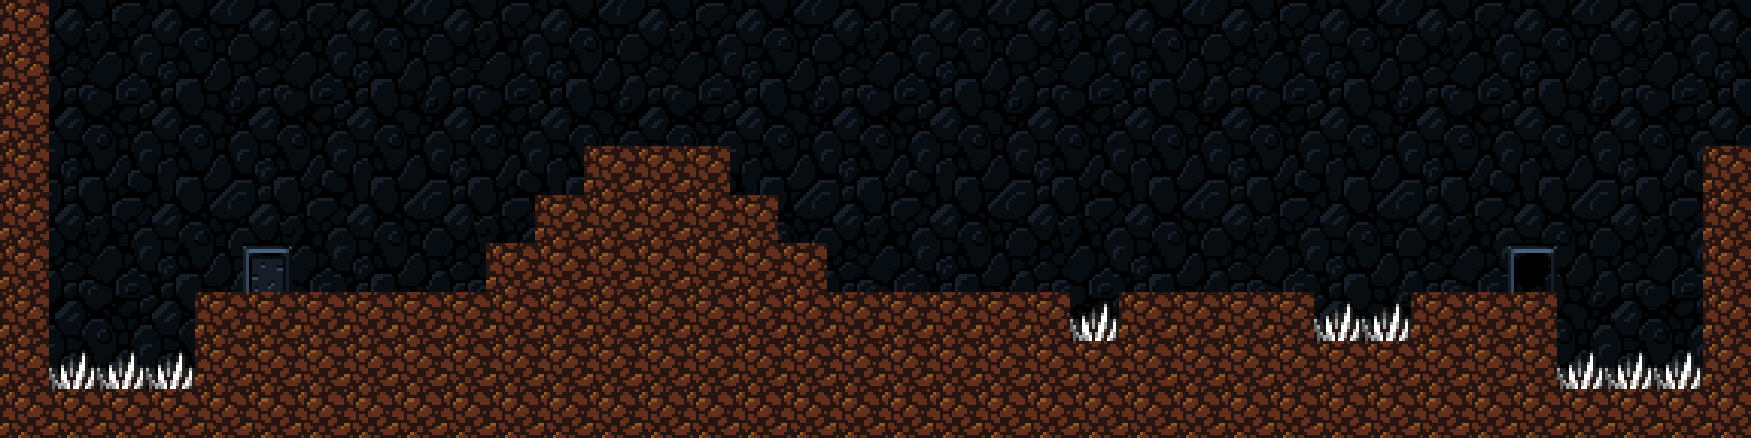
\includegraphics[width=\textwidth]{fig/levels/level1.pdf}
\caption{Cenário fácil, que explora o deslocamento horizontal do jogador.}
\label{fig:level1}
\end{figure}

O nível \textbf{médio}, além de explorar os elementos do nível \textit{fácil},
também requer que o jogador desloque-se \textbf{verticalmente}. Esse nível é
mais difícil que o \textit{fácil}, pois o jogador precisa \textbf{mudar de
direção} duas vezes. A figura \ref{fig:level2} mostra o nível médio, onde o
jogador deve partir da entrada localizada na plataforma mais acima e à
esquerda e chegar até a saída que se encontra no canto direito e abaixo.

\begin{figure}[H]
\centering
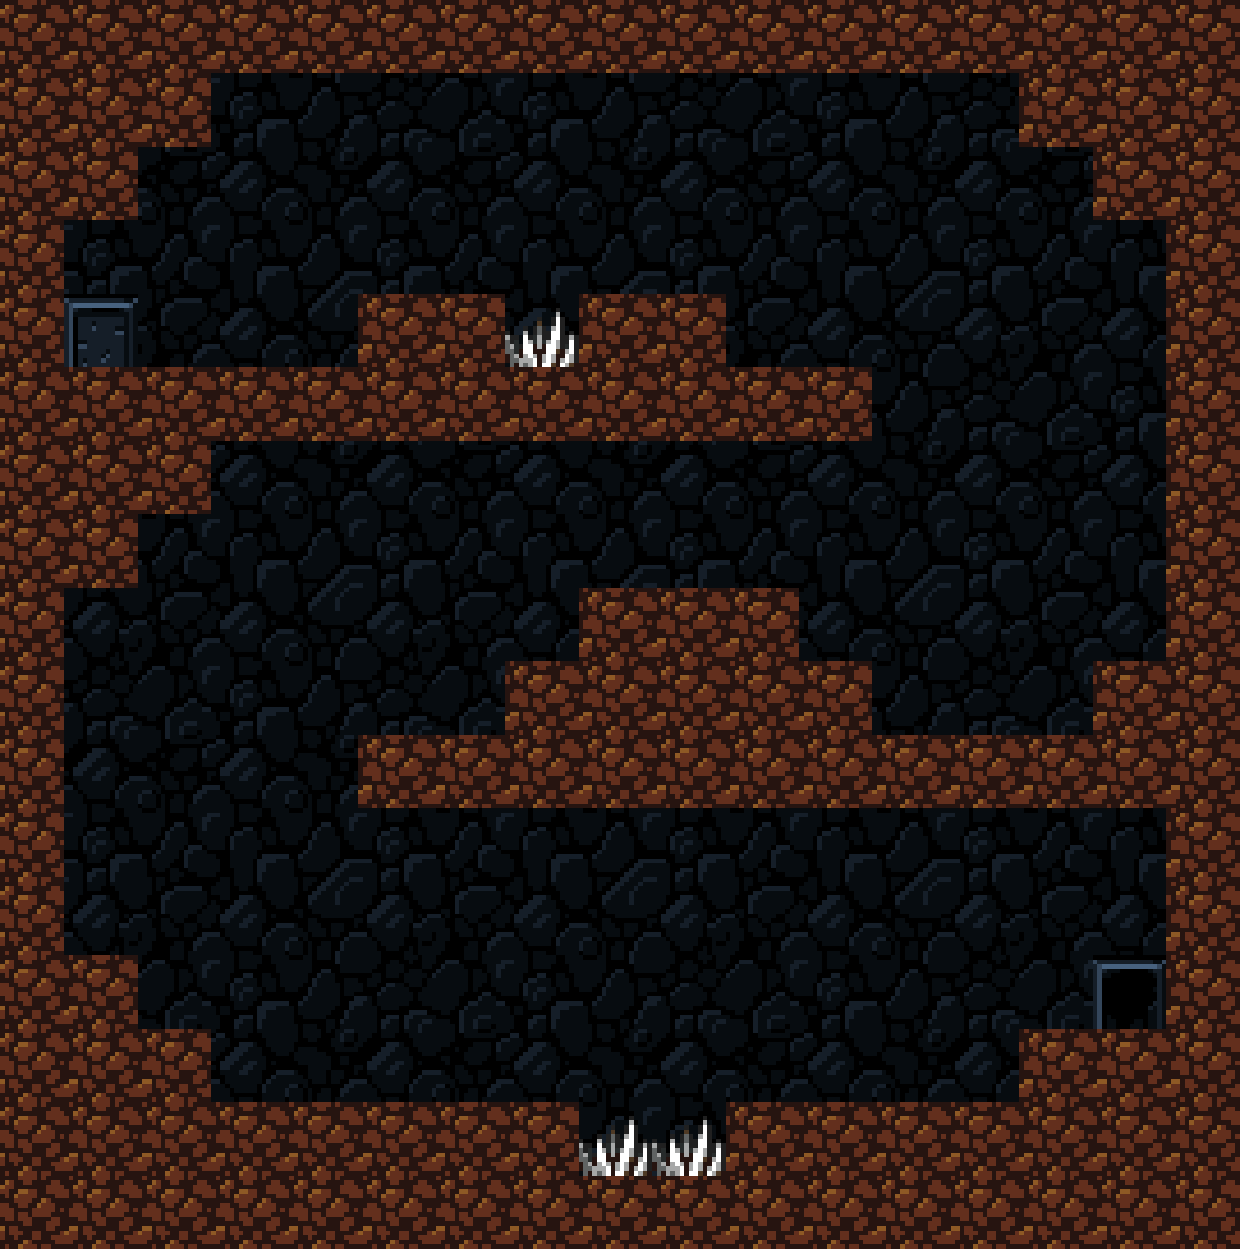
\includegraphics[width=\textwidth / 2]{fig/levels/level2.pdf}
\caption{Cenário médio, que explora o deslocamento horizontal e vertical do
    jogador, além de explorar a mudança de direção.}
\label{fig:level2}
\end{figure}

Para o nível médio, que conta com mais alguns desafios, estabelecemos os
seguintes \textbf{critérios de parada}:

\begin{itemize}
	\item \textbf{Número de execuções:} no máximo \textbf{10000} execuções.
	\item \textbf{Tempo de execução:} no máximo \textbf{20 segundos}.
\end{itemize}

O nível \textbf{difícil} é um nível gerado aleatóriamente pelo jogo. Mesmo sendo
gerado, é possível -- conforme a seção \ref{section:spelunky-procgen-path} --
atravessá-lo sem a necessidade de usar bombas, cordas ou outros equipamentos.
Este é o cenário mais interessante e desafiados deste trablaho.

\begin{figure}[H]
\centering
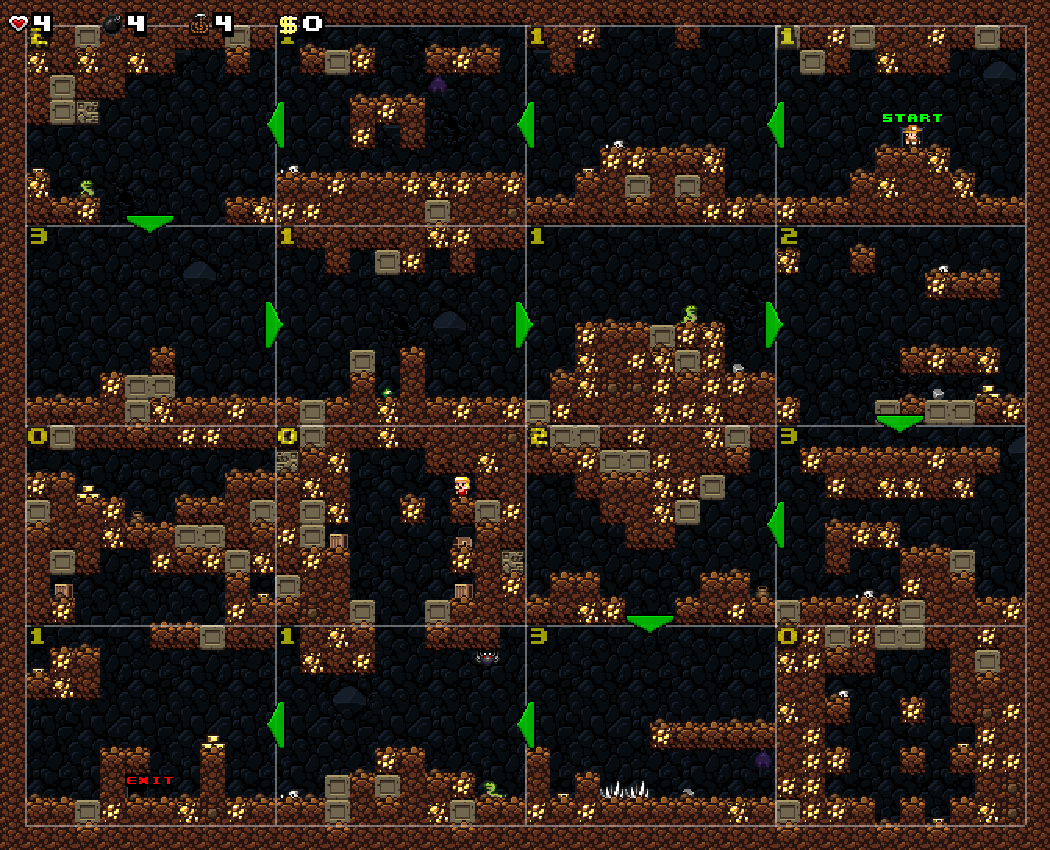
\includegraphics[width=\textwidth / 2]{fig/levels/level3.pdf}
\caption{Cenário difícil, extraido do gerador procedural de níveis do jogo.
	Alguns elementos (inimigos, tesouros, entre outros) foram removidos para
	limitar a dificuldade do cenário.}
\label{fig:level3}
\end{figure}


Por ser o cenário mais desafiador, estabelecemos os seguintes \textbf{critérios
de parada}:

\begin{itemize}
	\item \textbf{Número de execuções:} no máximo \textbf{20000} execuções.
	\item \textbf{Tempo de execução:} no máximo \textbf{90 segundos}.
\end{itemize}


\section{\label{section:scenarios-specific}Cenários Específicos}

Existem alguns desafios presentes em muitos níveis do jogo que não aparecem nos
cenários de testes convencionais. Estes desafios requerem a combinação de botões
em algum conjunto ou ordem específica. Visando explorar estes elementos,
elaboramos alguns cenários para testes de situações específicas.

Por serem cenários simplificados, elaboramos os seguintes \textbf{critérios de
parada} para todos eles:

\begin{description}
    \item [Número de execuções] no máximo \textbf{10000} execuções.
    \item [Tempo máximo de execução] no máximo \textbf{10 segundos} executando.
\end{description}

O cenário \textbf{extra 1}, exibido na figura \ref{fig:extra1}, conta com uma
escada que liga a plataforma inferior do jogo à plataforma superior. Portanto,
o jogador que deseja chegar até a porta de saída localizada na plataforma
superior deve fazer uso desta escada.

\begin{figure}[H]
\centering
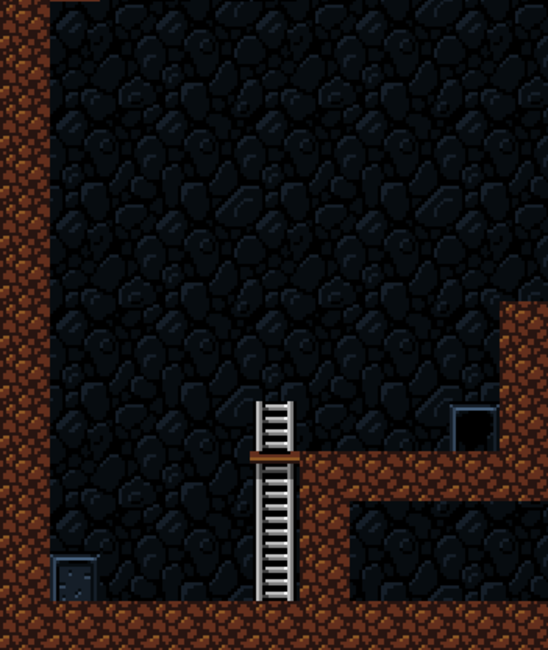
\includegraphics[width=\textwidth / 2]{fig/levels/extra1.pdf}
\caption{Cenário extra 1, que explora o uso de escadas por parte do jogador.}
\label{fig:extra1}
\end{figure}

Em alguns momentos, é necessário que o jogador se agarre à parede para atingir
locais mais elevados. Este é um problema interessante, pois é necessário que o
agente realize a combinação de ações de movimentação e salto. O nível
\textbf{extra 2} -- mostrado na figura \ref{fig:extra2} -- só pode ser vencido
caso o jogador salte, se agarre na parede e salte novamente, alcançando a
plataforma mais alta.

\begin{figure}[H]
\centering
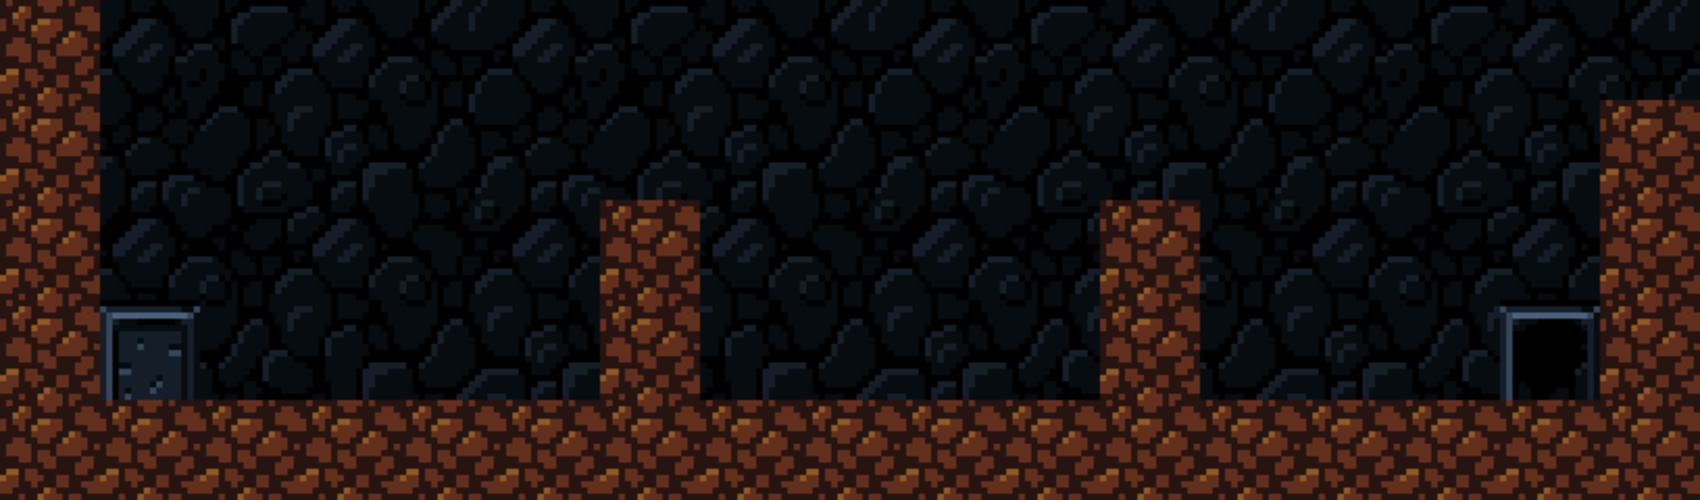
\includegraphics[width=\textwidth / 2]{fig/levels/extra2.pdf}
\caption{Cenário extra 2, que faz com que o jogador tenha que se agarrar à
    parede para vencer o nível.}
\label{fig:extra2}
\end{figure}

O jogador também conta com a ação de \textbf{correr}, fazendo com que seu
deslocamento pelo nível seja mais rápido. Além disso, quando o jogador corre, é
possível que este tenha uma impulsão maior no momento de saltar, sendo capaz de
superar buracos ou obstáculos mais compridos. De forma a explorar a corrida do
jogador, o nível \textbf{extra 3} -- representado na figura \ref{fig:extra3} --
só pode ser vencido caso o jogador pule os espinhos enquanto estiver correndo.

\begin{figure}[H]
\centering
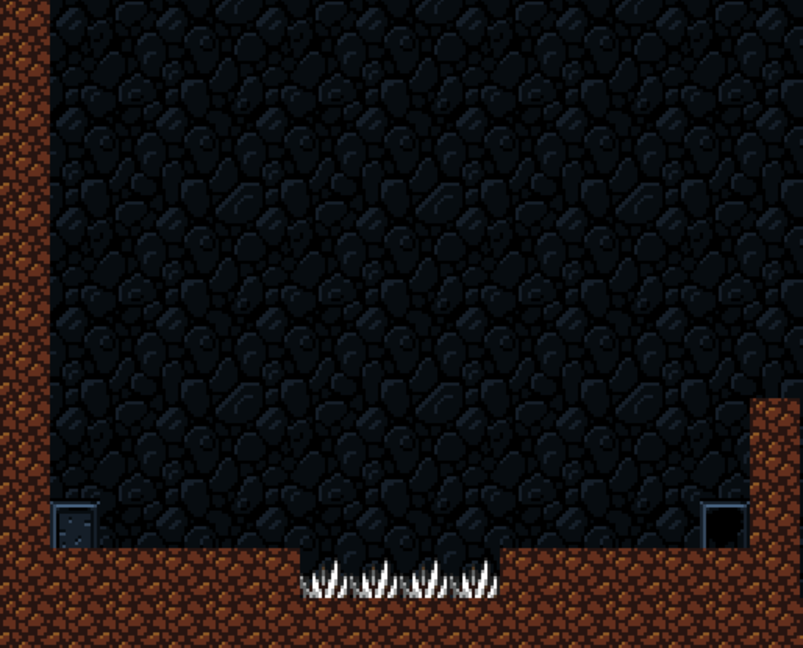
\includegraphics[width=\textwidth / 2]{fig/levels/extra3.pdf}
\caption{Cenário extra 3, que faz com que o jogador tenha que correr para
    vencer o nível.}
\label{fig:extra3}
\end{figure}
